\documentclass[11pt]{article}
\usepackage[T1]{fontenc}
\usepackage{lmodern}
\usepackage[margin=1.05in]{geometry}
\usepackage{amsmath,amssymb,amsthm,mathtools}
\usepackage{microtype}
\usepackage{xcolor}
\usepackage{tikz}
\usetikzlibrary{arrows.meta,decorations.pathreplacing,positioning}
\usepackage[hyphens]{url}
\usepackage[colorlinks=true,linkcolor=blue!45!black,citecolor=blue!45!black,urlcolor=blue!45!black]{hyperref}
\hypersetup{pdftitle={The geometric case of the Erdos similarity conjecture},pdfauthor={OpenAI}}
\newtheorem{theorem}{Theorem}[section]
\newtheorem{proposition}[theorem]{Proposition}
\newtheorem{lemma}[theorem]{Lemma}
\newtheorem{corollary}[theorem]{Corollary}
\theoremstyle{definition}
\newtheorem{definition}[theorem]{Definition}
\theoremstyle{remark}
\newtheorem{remark}[theorem]{Remark}
\newcommand{\R}{\mathbb R}
\newcommand{\N}{\mathbb N}
\newcommand{\Z}{\mathbb Z}
\newcommand{\Prob}{\mathbb P}
\newcommand{\E}{\mathbb E}
\newcommand{\1}{\mathbf 1}
\numberwithin{equation}{section}
\setlength{\emergencystretch}{2em}
\title{The geometric case of the Erd\H{o}s similarity conjecture}
\author{OpenAI}
\date{October 5, 2026}
\begin{document}
\maketitle
\begin{abstract}
We prove the geometric-progression case of the Erd\H{o}s similarity
conjecture. For every fixed $q\in(0,1)$ and every $\eta\in(0,1)$, we
construct a compact set $E_{q,\eta}\subseteq[0,1]$ of measure greater
than $1-\eta$ containing no nontrivial affine copy of
$\{q^n:n\ge1\}$, for any translation and either sign of nonzero dilation.
The set may depend on $q$; the result makes no simultaneous assertion
for different ratios.
\end{abstract}
\section{Introduction}\label{sec:introduction}

Let $m$ denote Lebesgue measure on $\R$. A set $A\subseteq\R$ is
\emph{measure universal} if every Lebesgue-measurable set of positive
measure contains a nontrivial affine copy
\[
 x+sA=\{x+sa:a\in A\},\qquad x\in\R,\quad s\in\R\setminus\{0\}.
\]
The Erd\H{o}s similarity conjecture \cite[Problem~4.33.7*]{Erdos1974Problems}
asserts that no infinite set is measure universal. We prove its
geometric-progression case. For
$q\in(0,1)$, write
\[
 G_q=\{q^n:n\in\N,\ n\ge1\}.
\]

\noindent\textit{Remark (notation).} $A$ denotes a subset of $\R$. In Theorem~\ref{thm:main}, Proposition~\ref{prop:periodic}, Lemma~\ref{lem:stability}, Lemma~\ref{lem:density}: As the argument of $\rho$, $A$ is Lebesgue-measurable and $1$-periodic, and $\rho(A)=m(A\cap[0,1))$. $x\in\R$ denotes the translation center in the affine points $x+sq^n$, or $x+tq^n$ for normalized dilation. In Lemma~\ref{lem:stability}: The assertion about earlier keys assumes $x\in\mathcal S$. In Lemma~\ref{lem:routing}, Lemma~\ref{lem:independent-tests}, Lemma~\ref{lem:conditional-scales}: $x\in\mathcal S$ is a stable center.


\begin{theorem}\label{thm:main}
For every $q\in(0,1)$ and $\eta\in(0,1)$, there is a compact set
$E_{q,\eta}\subseteq[0,1]$ with $m(E_{q,\eta})>1-\eta$ such that
\[
 \text{for every }x\in\R\text{ and }s\in\R\setminus\{0\},
 \quad x+sq^n\notin E_{q,\eta}\text{ for some integer }n\ge1.
\]
\end{theorem}

The avoiding set may depend on $q$. In particular, taking $q=1/2$
gives a compact set of arbitrarily large measure in $[0,1]$ avoiding
every signed affine copy of the dyadic sequence. The theorem treats
all geometric ratios, while the conjecture for arbitrary infinite
sets is a separate question.

\subsection{Background and related work}

Every finite pattern is measure universal. Indeed, if $F$ is finite
and $A$ is measurable with finite positive measure, continuity of
translations in $L^1$ gives
\[
 m\Bigl(\bigcap_{a\in F}(A-sa)\Bigr)\longrightarrow m(A)>0
 \qquad(s\to0).
\]
For an arbitrary positive-measure set, apply this observation to a
bounded subset of positive measure. The conjecture asks whether this
property always fails for infinite patterns.

Falconer~\cite{Falconer1984} and Eigen~\cite{Eigen1985} proved
nonuniversality for positive decreasing sequences $a_n\to0$ with
$a_{n+1}/a_n\to1$. Humke and Laczkovich
\cite[Theorems~1--2 and Corollary~1]{HumkeLaczkovich1998} developed a
finite covering characterization and further criteria in terms of
relative gaps. Kolountzakis~\cite[Theorem~3]{Kolountzakis1997} gave
a probabilistic criterion using large finite subsets with sufficiently
large normalized minimum gap. In the translation-invariant form of
Chleb\'ik~\cite[Theorem~15]{Chlebik2015}, a bounded infinite set is
nonuniversal if it contains finite subsets $a_1>\cdots>a_m$, of
arbitrarily large cardinality, for which
\[
 -\log\left(\frac{\min_{i<m}(a_i-a_{i+1})}{a_1-a_m}\right)=o(m).
\]
Geometric progressions do not satisfy this criterion. For distinct
powers of $q$, we have $a_{m-1}\le q^{m-2}a_1$ and
$a_1-a_m\ge(1-q)a_1$. Their normalized minimum gap is therefore at
most $q^{m-2}/(1-q)$, whose negative logarithm cannot be sublinear
in $m$.

\noindent\textit{Remark (notation).} $i\in\{1,\ldots,M\}$ indexes the ordered children of an internal vertex. In Proposition~\ref{prop:periodic}, Lemma~\ref{lem:density}, Lemma~\ref{lem:routing}, Lemma~\ref{lem:independent-tests}, Lemma~\ref{lem:conditional-scales}: Selector-bearing edges and local tests have $1\le i<M$; child $M$ is the default child and has no selector table.


Additive structure supplies another family of results.
Bourgain~\cite{Bourgain1987} proved that the sum of three infinite
sets is nonuniversal. Kolountzakis~\cite{Kolountzakis1997} treated
certain double sums, including $G_{1/2}+G_{1/2}$.
Mora Cuellar, Iosevich, Kulkarni, Rojas Aravena and
Yavicoli~\cite[Theorem~2]{MoraCuellarEtAl2026Twofold} proved that the
sum or difference of a geometric null sequence and any infinite set
is nonuniversal. Avoiding such a larger pattern does not imply
avoidance of the single geometric progression in Theorem~\ref{thm:main}.

Other results concern different classes of patterns or notions of
largeness. Iosevich, Kulkarni, Mora Cu\'ellar, Rojas Aravena and
Yavicoli~\cite[Theorem~1.5]{IKMRY2026Rajchman} prove nonuniversality
for sets supporting a probability measure whose Fourier transform
tends to zero at infinity. Such a measure is atomless, so the
hypothesis excludes countable sets
\cite[Proposition~4.1]{IKMRY2026Rajchman}.
Cruz, Lai and Pramanik~\cite[preprint, Corollary~1.2 and
Proposition~4.4]{CruzLaiPramanik2023} construct sets of Hausdorff
dimension one avoiding certain null sequences together with their
limit point; the subsets establishing that dimension have Lebesgue
measure zero. In a different direction, the theorem of Feng, Lai and
Xiong~\cite[preprint, Theorem~1.1]{FengLaiXiong2024} implies that
every $G_q$ embeds into every measurable set of positive measure by
a bi-Lipschitz map. The restriction to affine maps is therefore
substantive.

The proof below belongs to the probabilistic approach of
Kolountzakis~\cite{Kolountzakis1997}. Random cells, fixed-center
scale discretization, and integration of exceptional-center
probabilities also appear in Chleb\'ik~\cite[Section~5]{Chlebik2015}
and Kolountzakis--Papageorgiou~\cite[Section~3.1]{KolountzakisPapageorgiou2025};
the latter paper treats unbounded sequences. Solymosi~\cite[Section~3]{Solymosi2011Sparse}
and Tom~\cite{Tom2015} report incomplete dyadic constructions based on
random cells; Tom also considers nested dyadic intervals and tests
independent of the dilation. Our contribution is the
finite routing construction and its local control of the scale
count. We explain that mechanism next and give a self-contained proof.


\subsection{The proof mechanism}

We construct the open complement of the avoiding set. The intermediate
goal is an open, $1$-periodic set of arbitrarily small density that meets
$x+tG_q$ for every $x\in\R$ and every $t\in[1,2]$. A summable union
of its dilations and reflections then handles every nonzero scale;
Section~\ref{sec:periodic} gives this reduction. The remaining proof
uses only finite probability spaces and elementary measure theory.

\noindent\textit{Remark (notation).} $t\in[1,2]$ is the normalized dilation parameter in $x+tq^n$. In Lemma~\ref{lem:independent-tests}: The probability identity is evaluated for each $t$ fixed under the conditioning on $\xi$. In Lemma~\ref{lem:conditional-scales}: In the miss event, $t$ ranges existentially over $[1,2]$; each representative $t'\in\mathcal T_{x,\xi}$ used for the conditional probability bound is fixed on $\xi$ before remaining table entries are revealed.


For a fixed center and a fixed scale, many independent random cell
tests make a missed copy unlikely. The difficulty is to control all
scales at once. Recording every possible change at the finest grid
of a large construction can cost more than the failure probability
can afford. We arrange the tests on a finite ordered tree so that each
group of tests uses only the grids on one edge and in its child subtree.
Other parts of the tree may use much finer grids without increasing
the scale count for that group.

Each point is routed to a leaf by independent binary tables evaluated
at its grid cells. A node chooses the first child whose table returns
one, and chooses its last child by default if all earlier tables return
zero. The leaf has a separate table whose entries equal one with a
small probability $p$; this final table determines membership in the
random set and keeps its expected density equal to $p$.

\noindent\textit{Remark (notation).} $p\in(0,1)$ is the terminal-table Bernoulli parameter and the density budget used in the periodic construction. In Theorem~\ref{thm:main}: For each $k\in\Z$, the construction of $H_k$ uses $p=p_k=(\eta/64)4^{-|k|}$.


We assign a consecutive interval of sequence indices to each edge,
in the order that traverses an edge before its entire child subtree.
Gaps between these intervals make earlier routing decisions unchanged
by the translations associated with a later interval, except at a
small set of centers. Within the current interval, the translated
points use distinct entries of its own table. At the first default
on the center's route, the nondefault children therefore supply
many independent opportunities for a hit. Taking the tree sufficiently
deep makes the probability of having no default small.

The decisive length condition makes an edge's index interval at least
as long as the following gap and its child subtree together. Every
grid needed by a test from that interval then occurs within twice its
length. Thus the number of scale representatives depends on the
length of one interval, rather than on the resolution of the entire
tree. The branching number can be chosen so that the independent-test
failure probability beats this scale count.

For general $q$, we retain nested dyadic grids but choose their
resolutions comparable to $q^{-b}/(1-q)$ at index $b$. This gives
both the nesting needed to preserve earlier decisions and the
separation needed for fresh random entries. The branching number is
allowed to depend on $q$. These two adjustments let the same finite
routing mechanism accommodate any fixed geometric ratio.

\noindent\textit{Remark (notation).} $b$ ranges over the positive integers indexing $N_b$, $\Gamma_b$, and $J_b$. In Lemma~\ref{lem:separation}: In the proof's distance and cell-width estimates, $b=b_e$; the statement also considers every finer index $b\ge b_e$.


Finally, the construction may miss copies at a small closed set of
centers. An open neighborhood of those centers repairs every such
copy, because $x+tq^n$ tends to $x$. This converts the estimate for
exceptional centers into a statement valid at every center.
Section~\ref{sec:windows} constructs the grids and index intervals;
Section~\ref{sec:routing} proves the conditional independence of the
tests; and Section~\ref{sec:scales} controls all normalized scales
and completes the open-neighborhood repair.

\section{A periodic hitting set and the global deduction}
\label{sec:periodic}

Fix $q\in(0,1)$ for the rest of the proof. For a measurable,
$1$-periodic set $A\subseteq\R$, write
\[
 \rho(A)=m(A\cap[0,1)).
\]
We first restrict the dilation factor to $[1,2]$, while allowing every
real center. The following is the main construction.

\begin{proposition}\label{prop:periodic}
For every $p\in(0,1)$, there is an open $1$-periodic set $H\subseteq\R$
with $\rho(H)\le6p$ such that
\begin{equation}\label{eq:periodic-hitting}
 \text{for every }x\in\R\text{ and }t\in[1,2],
 \quad x+tq^n\in H\text{ for some integer }n\ge1.
\end{equation}
\end{proposition}

Sections~\ref{sec:windows}--\ref{sec:scales} prove this proposition.
We give its global consequence now, so that the subsequent construction
has a single normalized target. The summable measure budgets allow us
to use both expanding and contracting copies of the periodic set.

\begin{proof}[Proof of Theorem~\ref{thm:main}, assuming
Proposition~\ref{prop:periodic}]
For each $k\in\Z$, put
\[
 p_k=\frac{\eta}{64}\,4^{-|k|}
\]
and choose $H_k$ from Proposition~\ref{prop:periodic} with $p=p_k$.
Define
\begin{equation}\label{eq:global-open}
 C=\bigcup_{k\in\Z}\bigl(2^kH_k\cup(-2^kH_k)\bigr),
 \qquad E_{q,\eta}=[0,1]\setminus C.
\end{equation}
The set $C$ is open and symmetric under reflection, so $E_{q,\eta}$
is compact.

Each signed dilation $\pm2^kH_k$ is periodic with period $2^k$ and
has measure $2^k\rho(H_k)$ in one period. If $k\le0$, the interval
$[0,1]$ consists of exactly $2^{-k}$ periods. If $k>0$, it lies inside
a period interval of length $2^k$. In both cases,
\[
 m\bigl((\pm2^kH_k)\cap[0,1]\bigr)
 \le \max(1,2^k)\rho(H_k).
\]
Consequently,
\begin{align}
 m(C\cap[0,1])
 &\le12\sum_{k\in\Z}p_k\max(1,2^k)\notag\\
 &=\frac{12\eta}{64}
   \left(\sum_{j\ge1}4^{-j}+1+\sum_{k\ge1}2^{-k}\right)
 =\frac{7\eta}{16}<\eta.
 \label{eq:global-measure}
\end{align}
It follows that $m(E_{q,\eta})>1-\eta$.

For $s>0$, choose $k\in\Z$ and $t\in[1,2)$ with $s=2^kt$.
Apply Equation~\eqref{eq:periodic-hitting} to $H_k$ at the center
$2^{-k}x$. For some $n\ge1$ it gives
\[
 2^{-k}x+tq^n\in H_k,
 \qquad\text{hence}\qquad x+sq^n\in2^kH_k\subseteq C.
\]
For $s<0$, apply the same conclusion to $-x$ and $-s>0$ and reflect.
Thus every nontrivial affine copy of $G_q$ meets $C$ and is not
contained in $E_{q,\eta}$.
\end{proof}

The dyadic factors in Equation~\eqref{eq:global-open} only normalize
the dilation parameter. They do not change the index $n$ or require
any algebraic relation between $2$ and $q$.

\section{Grids, preorder windows, and stable centers}\label{sec:windows}

We now prepare the index windows used to find a hit at a normalized scale
$t\in[1,2]$.  Each edge of a finite ordered tree will carry one window.
We will bound the set of centers at which translations by $tq^n$ from a
given window can change earlier grid keys, and show that the translated
points take distinct keys at the edge's own resolution.
Throughout this section, $q\in(0,1)$ and the integers
$M\ge2$, $d\ge1$, $g\ge1$, and $r_0\ge1$ are arbitrary and fixed.

\noindent\textit{Remark (notation).} $M\ge2$ is a fixed integer giving the number of ordered children at each internal vertex of the complete tree. In Proposition~\ref{prop:periodic}: For the given $p\in(0,1)$ and $q\in(0,1)$, choose $M$ so that $\alpha:=p(M-1)/2>2\log(1/q)$. $d\ge1$ is the fixed integer height of the complete ordered $M$-ary tree. In Proposition~\ref{prop:periodic}: After choosing $M$, the height $d$ is chosen to satisfy $(1-2^{1-M})^d<p$. $g\ge1$ is a fixed integer giving exactly the number of unused indices between consecutive windows in preorder. In Proposition~\ref{prop:periodic}: After fixing the tree with $K$ edges, $g$ is chosen to satisfy $4Kc q^{g+1}<p$. $r_0\ge1$ is a fixed integer construction parameter prescribing the lower bound for all window lengths $r_h$. In Proposition~\ref{prop:periodic}: The construction chooses $r_0=r_*$, where $D_{M,q}(r)e^{-p(M-1)r/2}<p$ for every integer $r\ge r_*$. $r$ is a positive integer length parameter. In Lemma~\ref{lem:routing}, Lemma~\ref{lem:independent-tests}, Lemma~\ref{lem:conditional-scales}: In the local notation for an atom $\xi$ admitting a first default vertex $U$ of height $h$, $r=r_h$; this length is fixed under the conditioning on $\xi$. In Proposition~\ref{prop:periodic}: In the threshold choice, $r$ ranges over all integers $r\ge r_*$; when the conditional scale estimate is applied on a center-exposure atom, its length argument is $r=r_h\ge r_*$.


For each integer $b\ge1$, put
\[
 c=\frac{4}{1-q},\qquad
 N_b=2^{\lceil\log_2(cq^{-b})\rceil},\qquad
 \Gamma_b=N_b^{-1}\Z.
\]
The periodic grid key of $z\in\R$ is
$J_b(z)=\lfloor N_b\{z\}\rfloor$, where
$\{z\}=z-\lfloor z\rfloor$.  Thus the cells are closed on the left and
open on the right, and a boundary point belongs to the cell on its right.
We have
\begin{equation}\label{eq:grid-size}
 cq^{-b}\le N_b<2cq^{-b}.
\end{equation}
All $N_b$ are powers of two and are nondecreasing in $b$.  Consequently,
if $b'\ge b$, then $N_{b'}/N_b$ is an integer and
\[
 J_b(z)=\left\lfloor\frac{J_{b'}(z)}{N_{b'}/N_b}\right\rfloor.
\]
In particular, a finer key determines every coarser key.  This nesting
is the reason for retaining dyadic grids even when $q$ is not dyadic.

\noindent\textit{Remark (notation).} $b'$ is a positive integer grid index, ranging over $b'\ge b$ in the nesting relation and denoting the endpoint of the immediate predecessor of $W_e$ in the stability condition for a noninitial window.


\subsection*{Assigning the windows}

Take a complete ordered $M$-ary tree of height $d$, with leaves of height
$0$.  Write $P_1,\ldots,P_M$ for the children of an internal vertex $P$,
and $(P,i)$ for the edge from $P$ to $P_i$.  Let $K$ be the total number
of edges.  Order the edges in preorder: for each $i=1,\ldots,M$, list
$(P,i)$ and then all edges in the subtree rooted at $P_i$, in the same
recursive order.  An edge and its child subtree therefore form a
consecutive block in this list.

Assign an integer interval $W_e=[a_e,b_e]\cap\N$ to each edge, in
preorder, leaving exactly $g$ unused indices between consecutive
windows.  All edges leaving a vertex of height $h$ receive a window of
length $r_h$.  For an edge with a nonleaf child, we make its window at
least as long as the gap and the entire child subtree that follow it.
To specify these lengths from the leaves upward, write $\sigma_h$ for
the span, including gaps, of all windows in a subtree of height $h$.
At height $1$ there are $M$ windows and $M-1$ gaps, so we set
\[
 r_1=r_0,\qquad \sigma_1=Mr_1+(M-1)g,
\]
and, for $2\le h\le d$, choose
\[
 r_h=\max\{r_0,g+\sigma_{h-1}\}.
\]
At height $h\ge2$ there are $M$ blocks, each comprising one outgoing
window, a gap, and a child subtree.  Another $M-1$ gaps separate these
blocks, giving
\[
 \sigma_h=M(r_h+g+\sigma_{h-1})+(M-1)g.
\]
Choose the first starting index $n_0\ge1$ so that
$2q^{n_0}\le1/4$, and place all subsequent windows with the prescribed
lengths and gaps.  Attach to each edge $e$ the grid indexed by its window
endpoint $b_e$, and set
\[
 \mathcal N=\bigcup_e W_e.
\]

\noindent\textit{Remark (notation).} $h$ denotes vertex height in the complete tree of height $d$, with leaves of height $0$. In Lemma~\ref{lem:window-span}: $h$ is the height of the vertex from which $e$ leaves, so $1\le h\le d$. In Lemma~\ref{lem:routing}, Lemma~\ref{lem:independent-tests}, Lemma~\ref{lem:conditional-scales}: Where the local notation uses the first default vertex $U$, $h$ is its height, with $1\le h\le d$, and is fixed under conditioning on the center-exposure atom $\xi$. $\sigma_h$ is the deterministic span, including intervening gaps, of all windows in a subtree of height $h$, defined for $1\le h\le d$ by the stated recursion. $\mathcal N=\bigcup_e W_e$ is the finite union over all edges of the constructed tree, consisting of positive integer indices beginning at $n_0\ge1$, where $2q^{n_0}\le1/4$. In Proposition~\ref{prop:periodic}: $\mathcal N$ is the finite index collection used to define $R$; the indices used to hit the open neighborhood $V$ may instead be any sufficiently large integers $n\ge1$.


For $e=(P,i)$, let $b_e^*$ be the largest endpoint among $W_e$ and all
windows in the subtree rooted at $P_i$.  The recursive choice has the
following useful consequence.

\begin{lemma}[Span of an edge and its child subtree]\label{lem:window-span}
If $e=(P,i)$ leaves a vertex of height $h$, then
\begin{equation}\label{eq:window-span}
 b_e^*-a_e+1\le2r_h.
\end{equation}
\end{lemma}

\begin{proof}
If $h=1$, the child is a leaf, so $b_e^*=b_e$ and the span is $r_1$.
If $h\ge2$, preorder places the child's subtree immediately after
$W_e$, apart from one gap of length $g$.  The span is therefore
$r_h+g+\sigma_{h-1}$, which is at most $2r_h$ by the definition of
$r_h$.
\end{proof}

Figure~\ref{fig:window-block} shows the block appearing in the proof.
Thus the finest grid used anywhere in this block has its index at most
$2r_h-1$ beyond $a_e$.  This will control the number of grid boundaries
encountered as $t$ varies.  The gaps between windows serve a different
purpose: they control the bound on the density of centers at which a
translation from a later window can change an earlier key.

\begin{figure}[tb]
\centering
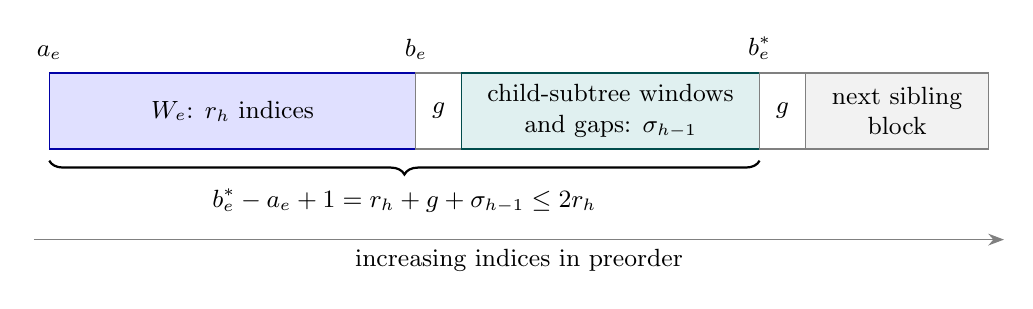
\begin{tikzpicture}[x=0.97cm,y=0.92cm,font=\small]
 \filldraw[fill=blue!12,draw=blue!65!black] (0,0) rectangle (4.8,1.05);
 \node at (2.4,.525) {$W_e$: $r_h$ indices};
 \draw[gray] (4.8,0) rectangle (5.4,1.05);
 \node at (5.1,.525) {$g$};
 \filldraw[fill=teal!12,draw=teal!60!black] (5.4,0) rectangle (9.3,1.05);
 \node[align=center] at (7.35,.525) {child-subtree windows\\and gaps: $\sigma_{h-1}$};
 \draw[gray] (9.3,0) rectangle (9.9,1.05);
 \node at (9.6,.525) {$g$};
 \filldraw[fill=black!5,draw=gray] (9.9,0) rectangle (12.3,1.05);
 \node[align=center] at (11.1,.525) {next sibling\\block};
 \node[above] at (0,1.1) {$a_e$};
 \node[above] at (4.8,1.1) {$b_e$};
 \node[above] at (9.3,1.1) {$b_e^*$};
 \draw[decorate,decoration={brace,mirror,amplitude=5pt},thick]
   (0,-.16)--(9.3,-.16);
 \node[below,align=center] at (4.65,-.42)
   {$b_e^*-a_e+1=r_h+g+\sigma_{h-1}\le2r_h$};
 \draw[-{Stealth[length=2mm]},gray] (-.2,-1.25)--(12.5,-1.25);
 \node[below] at (6.15,-1.25) {increasing indices in preorder};
\end{tikzpicture}
\caption{The block attached to an edge at height $h\ge2$, shown
schematically. The window length is at least the length of the following
gap and child-subtree span together. Thus the entire block has
at most twice the window length, regardless of where it occurs in the
tree. The next sibling block is outside this bound. At height $1$,
the child is a leaf and the block consists only of $W_e$.}
\label{fig:window-block}
\end{figure}


\subsection*{Preserving earlier keys}

Call $x\in\R$ \emph{stable} if, for every window $W_e$ other than the
first, writing $b'$ for the endpoint of its immediate predecessor,
\[
 (x,x+2q^{a_e}]\cap\Gamma_{b'}=\varnothing.
\]
Let $\mathcal S$ be the set of stable centers.  The left endpoint is
excluded because a translation to the right need not leave a grid cell
when it starts on that cell's left boundary; the right endpoint is
included because reaching the next boundary does change the key.

\begin{lemma}[Stability and earlier keys]\label{lem:stability}
The set $\mathcal S$ is measurable and $1$-periodic, and
\[
 \rho(\R\setminus\mathcal S)\le4Kc\,q^{g+1}.
\]
If $x\in\mathcal S$, $n\in W_e$, and $t\in[1,2]$, then every edge $f$
preceding $e$ in preorder satisfies
\begin{equation}\label{eq:stable-keys}
 J_{b_f}(x+tq^n)=J_{b_f}(x).
\end{equation}
\end{lemma}

\begin{proof}
For a fixed noninitial window, failure of its stability condition occurs
on the union of intervals
\[
 [\gamma-2q^{a_e},\gamma),\qquad \gamma\in\Gamma_{b'}.
\]
This is a measurable periodic set of density at most
\[
 2N_{b'}q^{a_e}
 \le4c\,q^{a_e-b'}
 =4c\,q^{g+1},
\]
where we used \eqref{eq:grid-size} and $a_e=b'+g+1$.  Summing over the
at most $K-1$ noninitial windows proves the stated density bound.

For the first window there are no earlier edges to consider.  Otherwise,
let $b'$ again be the endpoint of its predecessor, and suppose $x$ is
stable.  For $n\in W_e$ and $t\in[1,2]$, we have
$0<tq^n\le2q^{a_e}$.  Hence the segment from $x$ to $x+tq^n$ crosses
no boundary of $\Gamma_{b'}$, with a possible boundary at $x$ itself
assigned to the cell on its right.  It follows that
$J_{b'}(x+tq^n)=J_{b'}(x)$.  Every preceding edge $f$ has $b_f\le b'$,
so nesting gives \eqref{eq:stable-keys}.
\end{proof}

\subsection*{Separating the test points}

Earlier keys are now fixed at stable centers.  At the resolution attached
to the current edge, the center and its translated points instead have
distinct keys.  This second property holds at every center.

\begin{lemma}[Separation within one window]\label{lem:separation}
Fix an edge $e$, a center $x\in\R$, and a scale $t\in[1,2]$.  The points
\[
 \{x\}\ \cup\ \{x+tq^n:n\in W_e\}
\]
have pairwise distinct keys under $J_{b_e}$.  They also have pairwise
distinct keys under every $J_b$ with $b\ge b_e$.
\end{lemma}

\begin{proof}
Write $b=b_e$.  All the displayed points lie in
$[x,x+2q^{n_0}]$, an interval of length at most $1/4$.  Their pairwise
distances on the circle $\R/\Z$ therefore equal their ordinary real
distances.  The distance from $x$ to any translated point is
$tq^n\ge q^b$.  For $n<n'$ in $W_e$, the distance between the two
translated points is
\[
 t(q^n-q^{n'})=tq^n(1-q^{n'-n})\ge(1-q)q^b.
\]
On the other hand, \eqref{eq:grid-size} gives
\[
 \frac1{N_b}\le\frac{q^b}{c}
 =\frac{(1-q)q^b}{4}<(1-q)q^b.
\]
Two points with the same periodic key have circular distance less than
the cell width $1/N_b$.  Thus all the keys are distinct, including when
one of the points is a boundary point.  Distinctness persists at finer
resolutions because a finer key determines its coarser key.
\end{proof}

The random construction can consequently reuse all earlier decisions at
a stable center while consulting distinct entries for the points in the
current window.  We next use this distinction to obtain independent
opportunities for a hit.

\section{Random routing and independent tests}
\label{sec:routing}

Keep the tree, grids, and windows of Section~\ref{sec:windows}, and fix
\(p\in(0,1)\). We construct a random periodic set of expected density
\(p\), routing each point through the tree with one child at each internal vertex
designated as the default. When the route of a stable center makes a
default choice, the first such vertex supplies many tests for membership
of nearby points. We compute the probability of having no default choice
and show that, when the tests are available, their conditional failure
probability at each fixed scale decays exponentially in the window length.
The dependence on \(q\) enters through the grids and separation estimates
already established.

\subsection{The random tables}

For each edge \(e=(P,i)\) with \(i<M\), let
\[
 S_e:\{0,\ldots,N_{b_e}-1\}\longrightarrow\{0,1\}
\]
be a table of independent fair bits. Child \(M\) is the default child
and has no selector table. For each leaf \(L\), let \(b(L)\) be the
window endpoint of its incoming edge, and let
\[
 T_L:\{0,\ldots,N_{b(L)}-1\}\longrightarrow\{0,1\}
\]
be a table of independent Bernoulli-\(p\) bits. All entries of all
selector tables \(S_e\) and terminal tables \(T_L\) are mutually
independent. There are finitely many entries, so they define a finite
product probability space \(\Omega\), with probability \(\Prob\) and
expectation \(\E\). Write \(\mathcal A\) for the sigma-field generated
by all entries of all selector tables.

Given an outcome and \(z\in\R\), route \(z\) from the root as follows.
At an internal vertex \(P\), choose the first child \(P_i\), \(i<M\),
whose selector satisfies
\(S_{(P,i)}(J_{b_{(P,i)}}(z))=1\). If all these values are zero, choose
\(P_M\). Let \(L(z)\) denote the leaf reached and define
\begin{equation}
 \label{eq:random-set}
 B=\bigl\{z\in\R:
 T_{L(z)}(J_{b(L(z))}(z))=1\bigr\}.
\end{equation}
Every key is periodic, and every grid is refined by the finest grid in
the construction. Thus each realization of \(B\) is \(1\)-periodic
and is a union of finitely many half-open cells per period.

\noindent\textit{Remark (notation).} For each fixed $z\in\R$, $L(z)$ is the selector-dependent leaf reached from the root by the stated routing rule; it is $\mathcal A$-measurable and is fixed upon conditioning on $\mathcal A$. $B=\{z\in\R:T_{L(z)}(J_{b(L(z))}(z))=1\}$, with routing and terminal membership evaluated in the same table outcome, and each realization is $1$-periodic and a union of finitely many half-open grid cells per period. In Proposition~\ref{prop:periodic}: After the expectation estimates, one table outcome is fixed with $\rho(B^+)+\rho(R)\le5p$, and the subsequent construction uses its realization of $B$.


\begin{lemma}[Mean density]
 \label{lem:density}
The random set \(B\) in \eqref{eq:random-set} satisfies
\(\E\rho(B)=p\).
\end{lemma}

\begin{proof}
For fixed \(z\), conditioning on \(\mathcal A\) fixes
its leaf and terminal address. The terminal entry at that address still
has Bernoulli-\(p\) law, so \(\Prob(z\in B\mid\mathcal A)=p\).
Integration over one period, interchanged with the finite weighted sum
over \(\Omega\), gives
\[
 \E\rho(B)=\int_0^1\Prob(z\in B)\,dz=p.
\]
\end{proof}

\subsection{Exposing the center and routing local tests}

For a fixed center \(x\in\R\), expose its addressed entry in
\emph{every} selector table, including tables outside its route. Write
\begin{equation}
 \label{eq:center-exposure}
 \mathcal F_x=
 \sigma\bigl(S_e(J_{b_e}(x)):e=(P,i),\ i<M\bigr)
 \subseteq\mathcal A.
\end{equation}
An atom \(\xi\) of \(\mathcal F_x\) specifies all these entries and
has positive probability. Their addresses are deterministic once \(x\)
is fixed. On every atom, the remaining selector entries are therefore
independent fair bits, and all terminal entries retain their independent
Bernoulli-\(p\) laws.

\noindent\textit{Remark (notation).} $\xi$ is a fixed positive-probability atom of $\mathcal F_x$, specifying the addressed selector entry at $x$ in every selector table; conditioning on $\xi$ means conditioning on this event. In Lemma~\ref{lem:routing}, Lemma~\ref{lem:independent-tests}, Lemma~\ref{lem:conditional-scales}: $x$ is stable and $\xi$ admits a default choice on the route of $x$; its first default vertex $U$ and height $h$ are fixed on $\xi$.


The exposure determines the entire route of \(x\). If that route uses
a default child, let \(U\) be the first vertex where it does so.
Before conditioning on \(\mathcal F_x\),
\begin{equation}
 \label{eq:no-default}
 \Prob\bigl(\text{the route of \(x\) has no default choice}\bigr)
 =(1-2^{1-M})^d.
\end{equation}
Indeed, reveal the entries along the route one vertex at a time. At the
vertex reached, its \(M-1\) selector entries are independent fair bits,
since the preceding choices use only ancestor tables. The conditional
probability of a default is \(2^{-(M-1)}\). Multiplying the complementary
conditional probabilities over the \(d\) decisions proves the formula.

\noindent\textit{Remark (notation).} $U$ is the $\mathcal F_x$-determined first internal vertex at which the route of $x$ chooses the default child, defined only when that route has a default choice; on any atom $\xi$ admitting $U$, both $U$ and its height $h\in\{1,\ldots,d\}$ are fixed.


Now fix a stable center \(x\) and an atom \(\xi\) on which \(U\)
exists. Under this conditioning, \(U\) and its height \(h\) are fixed.
Put
\[
 r=r_h,\qquad e_i=(U,i)\quad(1\le i<M),\qquad
 y_n(t)=x+tq^n\quad(t\in[1,2]).
\]
All \(M-1\) selector values at \(x\) on these edges are zero. The
windows \(W_{e_i}\) will provide \((M-1)r\) possible hits.

\noindent\textit{Remark (notation).} $e_i=(U,i)$, $1\le i<M$, denotes an outgoing nondefault edge of the first default vertex $U$ of the center $x$; these edges are defined when $U$ exists and are fixed on an atom $\xi$ of $\mathcal F_x$ admitting $U$.


For \(i<M\), let \(L_i(z)\) be the leaf reached by routing \(z\)
starting at the child \(U_i\); if this child is a leaf, take
\(L_i(z)=U_i\). Define the local test
\begin{equation}
 \label{eq:local-test}
 Q_i(z)=S_{e_i}(J_{b_{e_i}}(z))\,
 T_{L_i(z)}(J_{b(L_i(z))}(z)).
\end{equation}
It consults only the selector on \(e_i\) and the tables in its child
subtree. The next lemma makes a successful local test a hit in \(B\).

\noindent\textit{Remark (notation).} For $z\in\R$ and $1\le i<M$, with $U$ fixed by an atom $\xi$ admitting a first default, $L_i(z)$ is the leaf obtained by routing $z$ from $U_i$ using the selectors in that child subtree, with $L_i(z)=U_i$ when $U_i$ is a leaf. For a stable center $x$ and a fixed atom $\xi$ admitting a first default vertex $U$, $Q_i$ is the table-dependent binary function on $\R$ defined by \eqref{eq:local-test}, indexed by $1\le i<M$, with $e_i=(U,i)$ and routing for $L_i(z)$ starting at $U_i$.


\begin{lemma}[Preservation of routing]
 \label{lem:routing}
Fix a stable center \(x\) and an atom \(\xi\) of \(\mathcal F_x\)
on which the first default vertex \(U\) exists. For every outcome in
\(\xi\), every \(i<M\), every \(n\in W_{e_i}\), and every
\(t\in[1,2]\), the route of \(y_n(t)\) reaches \(U\) and rejects its
children \(1,\ldots,i-1\). Consequently,
\begin{equation}
 \label{eq:local-hit}
 Q_i(y_n(t))=1\quad\Longrightarrow\quad y_n(t)\in B.
\end{equation}
\end{lemma}

\begin{proof}
At each strict ancestor \(P\) of \(U\), let \(a\) be the child index
chosen by \(x\). Since \(U\) is its first default vertex, \(a<M\).
The decision at \(P\) reads zeros at indices less than \(a\) and one
at \(a\). All these edges precede \(e_i\) in preorder, so their
selector values at \(y_n(t)\) equal those at \(x\) by
\eqref{eq:stable-keys}. Applying this observation successively from the
root shows that \(y_n(t)\) reaches \(U\). At \(U\), every edge
\((U,j)\) with \(j<i\) also precedes \(e_i\); its selector at
\(y_n(t)\) is therefore the exposed zero at \(x\).

If \(Q_i(y_n(t))=1\), its selector on \(e_i\) is one, so the actual
route takes child \(U_i\). Its continuation reaches the leaf
\(L_i(y_n(t))\), whose addressed terminal entry is one. This is exactly
the membership condition \eqref{eq:random-set}.
\end{proof}

\subsection{The exact failure probability at a fixed scale}

We now show that these tests are numerous enough to make a miss
unlikely. Their routes may share selector entries, so we first fix all
selectors and check that the resulting terminal addresses are distinct.
This order of conditioning keeps the dependence of the leaves on the
selectors explicit.

\begin{lemma}[Independent tests]
 \label{lem:independent-tests}
Fix a stable center \(x\) and an atom \(\xi\) of \(\mathcal F_x\)
on which the first default vertex \(U\) exists. Let \(h\) be its
height and \(r=r_h\), and define \(Q_i\) by \eqref{eq:local-test}.
For every fixed \(t\in[1,2]\),
\begin{equation}
 \label{eq:test-failure}
 \Prob\left(
 Q_i(y_n(t))=0\text{ for all }i<M,\ n\in W_{e_i}
 \,\middle|\,\xi\right)
 =(1-p/2)^{(M-1)r}.
\end{equation}
\end{lemma}

\begin{proof}
On the atom \(\xi\), the index set
\[
 \mathcal I=\{(i,n):1\le i<M,\ n\in W_{e_i}\}
\]
is fixed and has cardinality \((M-1)r\). For each pair put
\(A_{i,n}=S_{e_i}(J_{b_{e_i}}(y_n(t)))\).
For fixed \(i\), Lemma~\ref{lem:separation} gives pairwise distinct
keys for \(x\) and the points \(y_n(t)\), \(n\in W_{e_i}\), at
resolution \(b_{e_i}\). Thus the \(A_{i,n}\) use distinct entries of
their table and avoid its entry exposed at \(x\). Different \(i\)'s
use different tables. Conditional on \(\xi\), all \(A_{i,n}\) are
therefore independent fair bits.

\noindent\textit{Remark (notation).} $\mathcal I=\{(i,n):1\le i<M,\ n\in W_{e_i}\}$, with $e_i=(U,i)$ for the first-default vertex $U$, is fixed on each conditioning atom $\xi$ admitting a first default and has cardinality $(M-1)r_h$, where $h$ is the height of $U$. $A_{i,n}=S_{e_i}(J_{b_{e_i}}(y_n(t)))$ is defined for $1\le i<M$ and $n\in W_{e_i}$. In Lemma~\ref{lem:independent-tests}: For a stable center $x$, an atom $\xi$ of $\mathcal F_x$ admitting a first default, and a scale $t\in[1,2]$ fixed under this conditioning, the index set $\mathcal I=\{(i,n):1\le i<M,\ n\in W_{e_i}\}$ is fixed and has cardinality $(M-1)r_h$; its entries $A_{i,n}$ consult pairwise distinct selector entries, none exposed at $x$.


Next condition on \(\mathcal A\), the sigma-field of all selectors.
For each pair, its local leaf \(L_{i,n}=L_i(y_n(t))\) and terminal
address
\[
 \kappa_{i,n}
 =\bigl(L_{i,n},J_{b(L_{i,n})}(y_n(t))\bigr)
\]
are fixed. These addresses are distinct. If two child indices differ,
the leaves lie in disjoint child subtrees of \(U\), so their tables
differ. If the child indices agree but the leaves differ, the tables
again differ. Finally, suppose two different indices \(n,n'\) below
the same child select the same leaf \(L\). Its incoming edge is either
\(e_i\) itself or a later edge in that child subtree, so
\(b(L)\ge b_{e_i}\). The two points have different keys at resolution
\(b_{e_i}\), and nesting preserves this distinction at resolution
\(b(L)\). Their terminal addresses are distinct in this case as well.

\noindent\textit{Remark (notation).} For $1\le i<M$ and $n\in W_{e_i}$, $L_{i,n}=L_i(y_n(t))$ is the selector-dependent leaf reached by routing $y_n(t)$ from $U_i$. In Lemma~\ref{lem:independent-tests}: With $t$ fixed on $\xi$, conditioning further on $\mathcal A$ fixes $L_{i,n}$. For $1\le i<M$ and $n\in W_{e_i}$, $\kappa_{i,n}=(L_i(y_n(t)),J_{b(L_i(y_n(t)))}(y_n(t)))$ is a selector-dependent terminal address. In Lemma~\ref{lem:independent-tests}: With $t$ fixed on $\xi$, conditioning further on $\mathcal A$ fixes $\kappa_{i,n}$.


Consequently, for each realization of the selectors, the terminal
entries at all addresses \(\kappa_{i,n}\) are independent
Bernoulli-\(p\) variables. The pairs with \(A_{i,n}=0\) fail already;
each remaining pair fails precisely when its terminal bit is zero.
Hence, on \(\xi\),
\[
 \Prob\bigl(Q_i(y_n(t))=0\text{ for all }(i,n)\in\mathcal I
       \mid\mathcal A\bigr)
 =(1-p)^{\sum_{(i,n)\in\mathcal I}A_{i,n}}.
\]
Since \(\mathcal F_x\subseteq\mathcal A\), averaging over the
selectors conditional on \(\xi\) gives
\begin{align*}
 &\Prob\bigl(Q_i(y_n(t))=0\text{ for all }(i,n)\in\mathcal I
       \mid\xi\bigr)\\
 &\qquad=\E\left[(1-p)^{\sum_{(i,n)\in\mathcal I}A_{i,n}}
       \,\middle|\,\xi\right]
 =\prod_{(i,n)\in\mathcal I}\left(\frac12+\frac{1-p}{2}\right)
 =(1-p/2)^{(M-1)r}.
\end{align*}
\end{proof}

The estimate holds for every center-exposure atom admitting a default
and every scale fixed on that atom. Section~\ref{sec:scales} will use
the child-subtree endpoints \(b_{e_i}^*\) to select finitely many such
scales representing all \(t\in[1,2]\). Together with
\eqref{eq:no-default} and Lemma~\ref{lem:density}, this will control
misses while keeping the expected density small.

\section{All normalized scales and all centers}\label{sec:scales}

The independent tests of Section~\ref{sec:routing} control a fixed
scale at a fixed stable center.  We first make this estimate simultaneous
over $t\in[1,2]$, using only the grids that determine the local tests.
We then choose the construction parameters and cover the remaining
centers by a small open set.  The finite boundary-representative argument
has precedents in \cite[proof of Theorem~15]{Chlebik2015} and
\cite[Section~3.1]{KolountzakisPapageorgiou2025}.

\begin{lemma}[Conditional control of all normalized scales]
\label{lem:conditional-scales}
Fix $p\in(0,1)$ and the construction parameters $M,d,g,r_0$ of
Sections~\ref{sec:windows} and~\ref{sec:routing}.
Let $x\in\mathcal S$ be a stable center, and let $\xi$ be an atom of
the center-exposure field $\mathcal F_x$ on which the route of $x$
uses a default edge.  If its first default occurs at a vertex $U$ of
height $h$, put $r=r_h$ and
\begin{equation}\label{eq:scale-count}
 D_{M,q}(r)=4+2(M-1)r\bigl(1+2c q^{-2r}\bigr).
\end{equation}
Then
\begin{equation}\label{eq:conditional-scales}
 \Prob\!\left(
  \exists t\in[1,2]\ \forall n\in\mathcal N:\
  x+tq^n\notin B\ \middle|\ \xi
 \right)
 \le D_{M,q}(r)e^{-p(M-1)r/2}.
\end{equation}
\end{lemma}

\begin{proof}
On the atom $\xi$, the vertex $U$ and its outgoing edges
$e_i=(U,i)$, $1\le i<M$, are fixed.  Recall that
$Q_i(z)$ tests the selector on $e_i$ and terminal membership after
routing from $U_i$.  Every table used by this test belongs to $e_i$
or the subtree below it.  By nesting of the grids, for every realization
of the tables, $Q_i(z)$ is determined by the single key
$J_{b_{e_i}^*}(z)$.

For each $i<M$ and $n\in W_{e_i}$, record the values of $t\in[1,2]$
for which $y_n(t)=x+tq^n$ lies on the lattice
$\Gamma_{b_{e_i}^*}$.  The segment traversed by $y_n$ has length
$q^n$, so the number of recorded values is at most
\begin{equation}\label{eq:local-boundaries}
 1+q^nN_{b_{e_i}^*}
 \le 1+2c q^{-2r}.
\end{equation}
Here we used~\eqref{eq:grid-size} and the block-span bound
$b_{e_i}^*-a_{e_i}+1\le2r$ from
Lemma~\ref{lem:window-span}.

Combine these lists, add $1$ and $2$, and retain the distinct values in
increasing order.  Let $\mathcal T_{x,\xi}$ consist of these values
together with one midpoint between each consecutive pair.  There are
$(M-1)r$ pairs $(i,n)$, and hence
\[
 |\mathcal T_{x,\xi}|\le D_{M,q}(r).
\]
This set depends only on $x$, the deterministic windows and grids, and
the vertex $U$ determined by $\xi$; it is fixed before any remaining
table entries are revealed.  For every realization of those entries,
the entire vector
\[
 \bigl(Q_i(y_n(t)):\ i<M,\ n\in W_{e_i}\bigr)
\]
is constant on each open interval between consecutive recorded values.
Every boundary value is represented separately, so the half-open cell
convention causes no loss at a boundary or at an endpoint of $[1,2]$.

\noindent\textit{Remark (notation).} $\mathcal T_{x,\xi}$ is a finite subset of $[1,2]$ determined solely by $x$, the deterministic windows and grids, and the first default vertex $U$ determined by $\xi$, and is fixed conditional on $\xi$ before any remaining table entries are revealed.


If some $t$ misses $B$ at all indices in $\mathcal N$,
Lemma~\ref{lem:routing} implies that all these local tests fail at $t$.
They therefore also fail at some $t'\in\mathcal T_{x,\xi}$.
Each such $t'$ is a fixed real number under the conditioning on $\xi$,
so Lemma~\ref{lem:independent-tests} applies to it.  Taking a union
bound and using~\eqref{eq:test-failure} gives
\[
 \Prob\!\left(
  \exists t\in[1,2]\ \forall n\in\mathcal N:\
  x+tq^n\notin B\ \middle|\ \xi
 \right)
 \le |\mathcal T_{x,\xi}|(1-p/2)^{(M-1)r},
\]
which proves~\eqref{eq:conditional-scales}.
\end{proof}

The bound uses the last grid in each edge and descendant block.
Its resolution is controlled by that edge's window length through
\eqref{eq:window-span}.  Using the finest grid of the whole construction
would discard this control and would not give~\eqref{eq:scale-count}.

\begin{proof}[Proof of Proposition~\ref{prop:periodic}]
Fix $p\in(0,1)$.  We now specify the parameters that were left arbitrary
in the preceding construction.  Choose an integer $M\ge2$ such that
\begin{equation}\label{eq:branching-choice}
 \alpha:=\frac{p(M-1)}2>2\log(1/q).
\end{equation}
Next choose an integer $d\ge1$ satisfying
\[
 (1-2^{1-M})^d<p.
\]
For the resulting tree, let $K$ be its number of edges and choose an
integer $g\ge1$ such that
\[
 4Kc q^{g+1}<p.
\]
Finally, by~\eqref{eq:branching-choice},
\[
 D_{M,q}(r)e^{-\alpha r}
 =O\!\left(r e^{-(\alpha-2\log(1/q))r}\right)
 \longrightarrow0.
\]
Thus there is an integer $r_*\ge1$ such that
\begin{equation}\label{eq:window-length-choice}
 D_{M,q}(r)e^{-p(M-1)r/2}<p
 \qquad\text{for every integer }r\ge r_*.
\end{equation}
Construct the windows with $r_0=r_*$ and the chosen $M,d,g$, and form
the random set $B$ of Section~\ref{sec:routing}.

Fix any stable center $x$.  By~\eqref{eq:no-default}, the probability
that its route has no default is less than $p$.  On each atom of
$\mathcal F_x$ for which a default occurs,
Lemma~\ref{lem:conditional-scales} and~\eqref{eq:window-length-choice}
bound the conditional probability of a miss at some normalized scale
by $p$, since every $r_h\ge r_*$.  Summing over the center-exposure
atoms yields
\begin{equation}\label{eq:stable-miss}
 \Prob\!\left(
  \exists t\in[1,2]\ \forall n\in\mathcal N:\
  x+tq^n\notin B
 \right)\le2p
 \qquad(x\in\mathcal S).
\end{equation}
The probability space is finite, so this event is measurable even
though its definition quantifies over all $t\in[1,2]$.

It remains to turn this estimate at each center into a set that works
at every center. Open-neighborhood repair for null sequences is explicit
in Tom~\cite[Lemma~0.2]{Tom2015}; see also
Chleb\'ik~\cite[Section~3, final remark; Proposition~1(vi), (viii)]{Chlebik2015}.
We implement it with open neighborhoods, which contain sufficiently
late translated points because $tq^n\to0$.
For each table outcome, enlarge the finitely many
selected cells per period to an open periodic set $B^+\supseteq B$
with
\[
 \rho(B^+)\le\rho(B)+p.
\]
For that outcome define the set of centers still missed by the finite
collection of indices:
\begin{equation}\label{eq:exceptional-centers}
 R=\left\{x\in\R:\ \exists t\in[1,2]\ \forall n\in\mathcal N,
                   \ x+tq^n\notin B^+\right\}.
\end{equation}
This is a closed periodic set.  Indeed, on the circle $\R/\Z$ it is
the projection of the closed set
\[
 \left\{(x,t)\in(\R/\Z)\times[1,2]:
       x+tq^n\notin B^+\ \text{for all }n\in\mathcal N\right\}
\]
in a compact product.  In particular, its density is defined.

\noindent\textit{Remark (notation).} For each table outcome, $B^+$ is an open $1$-periodic enlargement of that outcome's set $B$, satisfying $B\subseteq B^+$ and $\rho(B^+)\le\rho(B)+p$. For each table outcome and its chosen enlargement $B^+$, $R=\{x\in\R:\exists t\in[1,2]\ \forall n\in\mathcal N,\ x+tq^n\notin B^+\}$ is a closed $1$-periodic set of centers.


Since $B\subseteq B^+$, membership of a fixed stable center in $R$
implies the event in~\eqref{eq:stable-miss}.  Lemma~\ref{lem:stability}
and the choice of $g$ give $\rho(\R\setminus\mathcal S)<p$.
Integrating the probability bound over one period therefore gives
\[
 \E\rho(R)
 =\int_0^1\Prob(x\in R)\,dx
 \le2p\rho(\mathcal S)+\rho(\R\setminus\mathcal S)
 \le3p.
\]
Also $\E\rho(B^+)\le2p$ by Lemma~\ref{lem:density}.
Choose a table outcome for which
\[
 \rho(B^+)+\rho(R)\le5p.
\]
Outer regularity on the circle supplies an open periodic set
$V\supseteq R$ with $\rho(V)\le\rho(R)+p$.
Then $H=B^+\cup V$ is open and periodic, and
\[
 \rho(H)\le\rho(B^+)+\rho(R)+p\le6p.
\]

\noindent\textit{Remark (notation).} $V$ is an open $1$-periodic superset of $R$, chosen after fixing a table outcome satisfying $\rho(B^+)+\rho(R)\le5p$, with $\rho(V)\le\rho(R)+p$.


To verify the hitting property, fix $x\in\R$ and $t\in[1,2]$.
If $x\notin R$, the definition of $R$ gives an index $n\in\mathcal N$
with $x+tq^n\in B^+\subseteq H$.
If $x\in R$, then $x\in V$ and $V$ is open, so
$x+tq^n\in V\subseteq H$ for all sufficiently large $n$ because
$tq^n\to0$.  These latter indices need not lie in $\mathcal N$;
the required conclusion allows every $n\ge1$.  Thus every center and
every normalized scale has a hit, proving the proposition.
\end{proof}

\bibliographystyle{alpha}
{
\raggedright
\bibliography{references}
}
\end{document}

\noindent\textit{Remark (notation).} $n$ is a positive integer indexing the power $q^n$. In Lemma~\ref{lem:stability}, Lemma~\ref{lem:separation}: The translated points are indexed by $n\in W_e=[a_e,b_e]\cap\N$ for the edge $e$ under consideration. In Lemma~\ref{lem:routing}, Lemma~\ref{lem:independent-tests}: For each $1\le i<M$, the local tests use $n\in W_{e_i}$, where $e_i=(U,i)$ is fixed on $\xi$. In Lemma~\ref{lem:conditional-scales}: The simultaneous miss event ranges over $n\in\mathcal N=\bigcup_e W_e$; the local tests used in its proof range over $n\in W_{e_i}$ for each $1\le i<M$.

